\section{Trying to climb into M2}

\begin{quote} Incompetence, bravery and no luck. \end{quote}



\begin{marginsurvey}
\checkoddpage \ifoddpage \forcerectofloat \else \forceversofloat \fi
\centering
 \frame{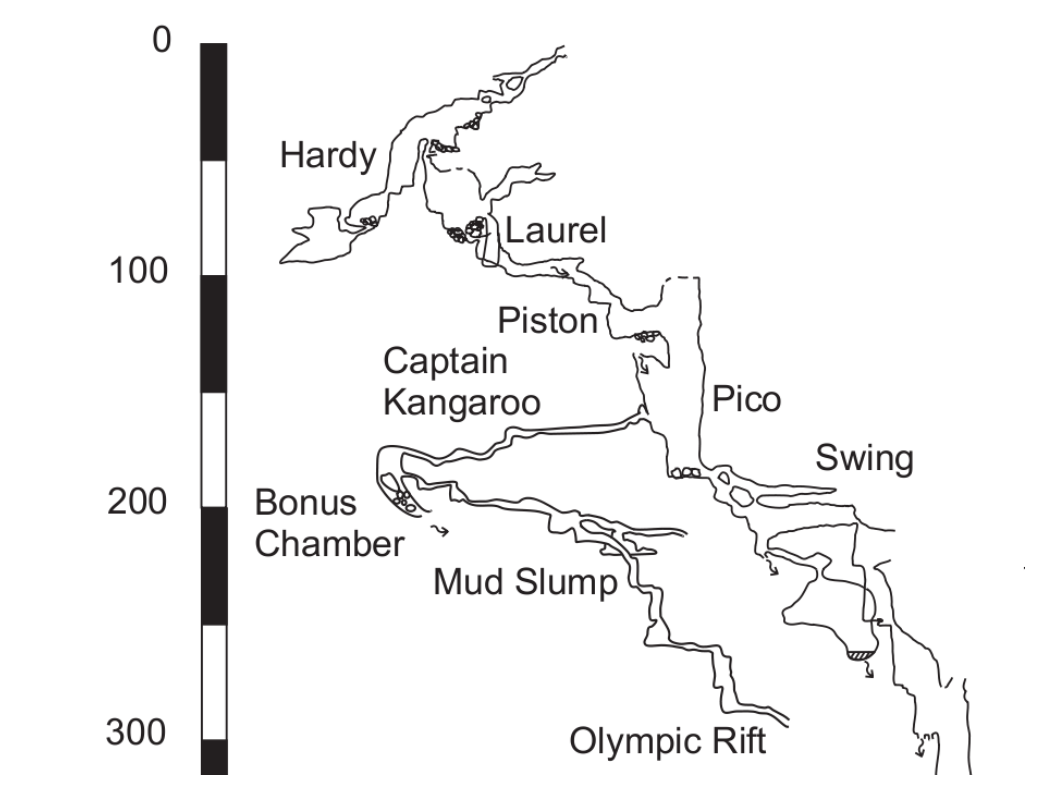
\includegraphics[width=\linewidth]{2008/m2_climb/cptkpre2008_bcra_2008.pdf.png}} 
 \caption[2007 Captain Kangaroo Survey]{The \protect\passage{Captain Kangaroo} branch was the subject of 2008's major exploratory efforts.}
 \label{cptk pre2008 survey}
\end{marginsurvey}


Our main aim in 2008 was to discover the connection between \passage{M2}
and \passage{Gardeners' World}, a feat which would heap honor on the
shoulders of who discovered it. 2008 was my first year of caving in
Slovenia and I was \textit{very keen}. I dreamed of my shoulders baring
the honor of the great discovery and did all I possibly could to be on
the right trip at the right time. I took part in a few of the rigging
trips down \passage{M2} and was amazed by alpine caving on \passage{Migovec}: the
truly huge pitches, the dry nature of the caving, could not wait for
more ``pushing''. At the time, the Bivi rumour machine had determined
the most likely way to find the connection was to explore the area
around \passage{Kill'em All} in \passage{Captain Kangaroo}. This side branch
of \passage{Vrtnarija} had been pushed the previous year by Rik and was
infamous: uncharacteristically tight and twatty, rigged sparsely and
badly, a total nightmare.


   \margininbox{Captain Kangaroo}{
     \begin{itemize}
    \item Clewin Griffiths    
    \item James Kirkpatrick
    \end{itemize}}{\explo}


My first pushing trip in \passage{Captain Kangaroo} was with Clewin. The
deeper you get into \passage{Captain Kangaroo} the more ridiculous the
rigging was, with plenty of dodgy climbs waiting to dislocate your
shoulder or break your ankle. The cherry on the cake was at the time
\passage{Kill'em All}, \bignote{the most insane piece of rigging I have ever been
exposed to}.

The pitch head is at the end of a tight rift. The original rigging
consisted of a Y-hang in the main shaft, roughly half a meter below the
entrance rift. The only way to get on the rope was to clip in and drop
on the rope, possibly with a forward roll. The only way to get out was
to clip the Y-hang with long cows tails, stand on the knot, wedge
yourself into the rift and unclip. In retrospect criminally dangerous
and terrifying, but at the time I thought this must be ``expedition
rigging'' and took it in my stride. On the way out we bumped into Jarv
and Paul who had rerigged large sections of the cave making it safer, by
the end of the year the cave was more or less sensible. On that day
Clewin and I pushed the main lead down, rigged two small pitches. I had
my first taste of caving exploration and I loved it. Game on!

\begin{marginfigure}
\checkoddpage \ifoddpage \forcerectofloat \else \forceversofloat \fi
\centering
 \frame{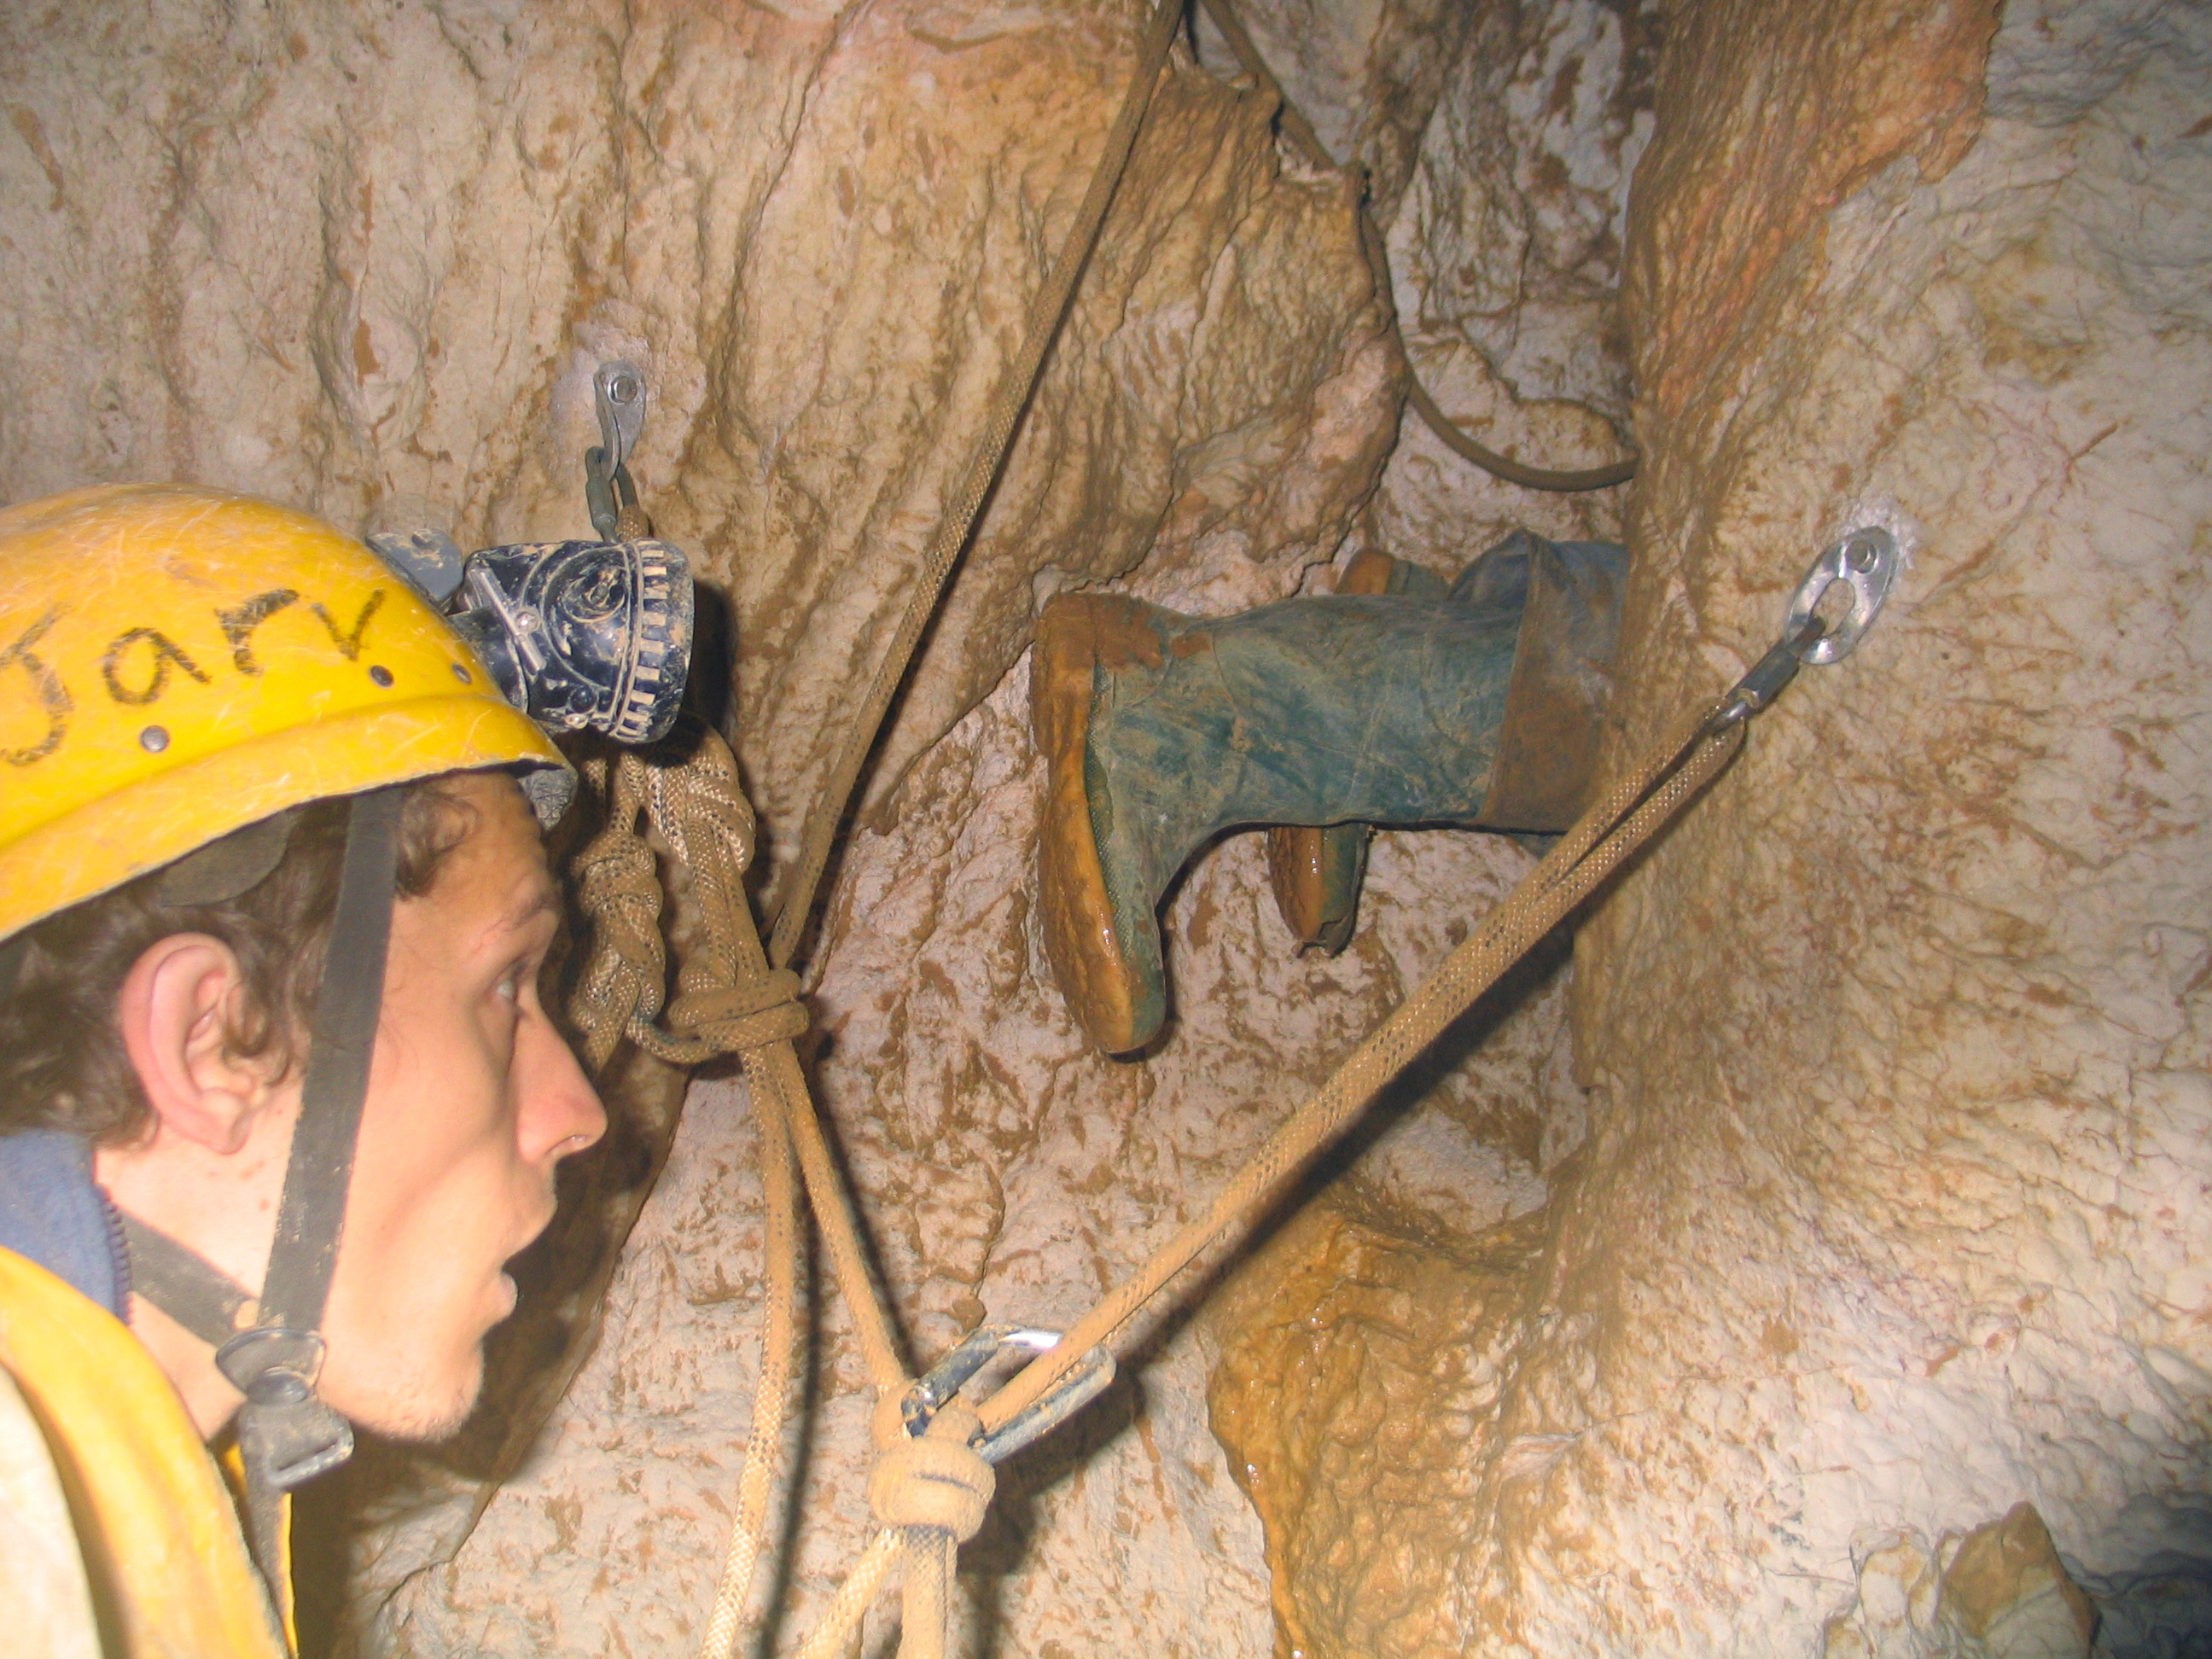
\includegraphics[width=\linewidth]{2008/m2_climb/2009-08-06-12.46.22 - Jarvist Frost - Canon Powershot G5 - Mikes wellies disappearing into the old killem all pitch head--orig.jpg}} 
 \caption{The pitch head of \protect\passage{Kill'em All} in 2009. \pic{Jarvist Frost}}
 \label{Kill em all wellies}
\end{marginfigure}

\margininbox{Cheesecake}{
     \begin{itemize}
    \item Gergely Ambrus
    \item Jarvist Frost
    \item James Kirkpatrick
    \end{itemize}}{\explo}


The trip with Clewin had already brought the bottom of the cave too deep
for the expected position of the closest point to \passage{M2}. I had
somehow developed a reputation as a `climber' and decided to have a go
at climbing into a side passage at the top of \passage{Kill'em All}. This
required an easy slabby climb halfway up the pitch. We added a bolt half
way down the pitch from which Gergely belayed me. In order to protect
the climb I had some very long 8 mm rawl bolts, a rock pecker and a
bunch of slings. I had tried out the rock pecker on the surface, but
found it much less easy to use whilst climbing, hammering away, the legs
a bit weak with fear of falling, footholds feeling precarious in the big wellies, feeling I would knock myself off the wall\ldots{} I bottled it,
abandoned a very poor bolt, slung a sling around a spike and free
climbed the short slab. A very easy climb (maybe Mod?) but nevertheless
terrifying. I think that Gergely's singing helped a lot. At the time it
felt like a great achievement. But it did not lead to the connection.


   \margininbox{Traverse above Primula}{
     \begin{itemize}
    \item James Kirkpatrick
    \item Izi Možir
    \end{itemize}}{\explo}


Climbing with a rock pecker was too scary, so the next time Izi and I
took an electric drill. It weighed a hell of a lot going through
\passage{Captain Kangaroo}, but it would make climbing the traverse above
\passage{Primula} a walk in the park. Unfortunately once we arrived, the
drill would not work. Bogus. Plan B: hammer in a spit and belay me
across. This also failed, due to the rock being very rotten. Plan C: use
a natural for the belay and then free climb. While Izi slung some
boulders and backed up to the rope above, I scoped the climb. Doable.
There is a sort of foothold halfway along but it is total commitment --
a long step. \bignote{The traverse was on the limit of the delicate climbing that can be done in full caving gear}, I reached the rift at the far end of
the traverse, wedged myself in and hammered the fastest spit I have ever
placed. Once secure, I considered the way on. The rift was going
slightly up and was totally blocked. No way on. But another crap
inducing climb, and another step to make me less Keen!

The highlight of that years caving for me was actually a trip in the
bottom of \passage{Captain Kangaroo} with Izi\sidenote{see later in this chapter}. On that trip we discovered
\passage{Dark Tranquillity}. It was the first proper pitch I pushed and the
buzz was incredible. I remember sitting at the top discussing with Izi
how it would rigged. I was apprehensive of screwing up, but he made it
clear he trusted me.

\begin{marginfigure}
\checkoddpage \ifoddpage \forcerectofloat \else \forceversofloat \fi
\centering
 \frame{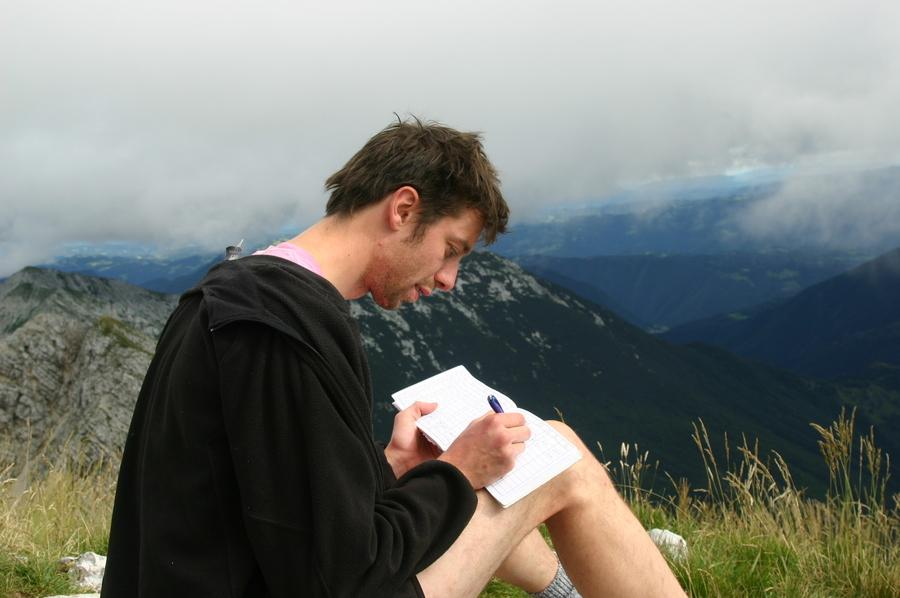
\includegraphics[width=\linewidth]{2008/m2_climb/Gergely Ambrus - DSLR - img_4941--orig.jpg}} 
 \caption{JKP writing notes on the surface. \pic{Gergely Ambrus}}
 \label{JKP sunset notes}
\end{marginfigure}

Somehow the expedition ends.

\begin{enumerate}
\def\labelenumi{\arabic{enumi}.}
% \tightlist
\item
  I am not upset at not having found the Connection.
\item
  I am glad that I had some fun pushing trips.
\item
  I am grateful I did not get hurt, or hurt my caving partners.
\item
  I am proud of having another person trusting me.
\item
  I am now a lot less Keen, know a thing or two about Bivi rumours. But
  it would take a few more broken drill carries to make me wizen up
  electrically!
\end{enumerate}

\name{James Kirkpatrick}
